\chapter{Planteamiento e introducción teórica}

El siguiente diagrame en bloques sintetiza las distintas etapas de la fuente, Desde la entrada de
$220V$ en CA hasta llegar a la tension en CC a la salida.

\begin{figure}[h]
  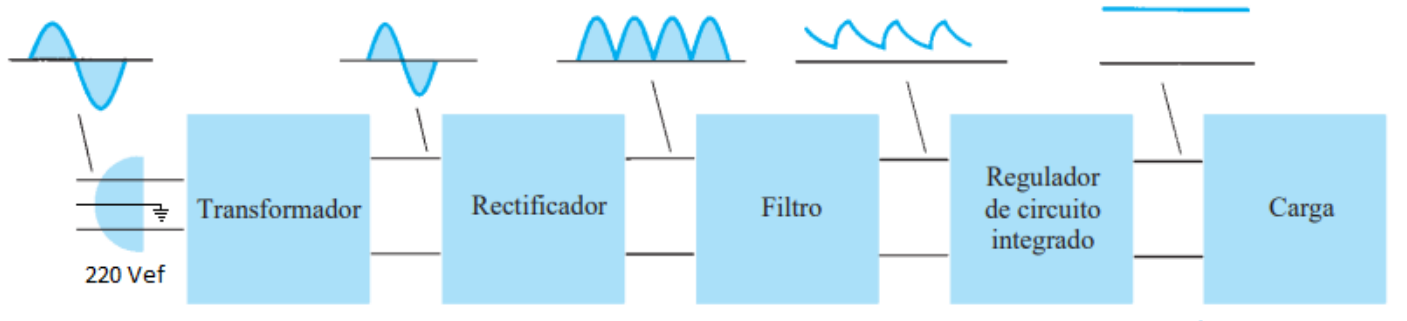
\includegraphics[width=0.95\textwidth]{images/diagramaBloques.png}
  \caption{Diagrame en bloques}
\end{figure}

A contunuación, se explica detaladamente cada uno de estos bloques.

\section{Transformador}

El transformador tiene dos funciones:
\begin{itemize}
  \item Aislar galvánicamente el circuito de la red electrica.
  \item Reducir la tension de entrada al valor necesario para la fuente.
\end{itemize}

\begin{circuitikz}
  \draw (0,0) to [sV] ++(0,2) -- ++(1,0)
  node[transformer core, circuitikz/inductors/coils=6,
  anchor=A1](T){};
  \draw (T.A2) -| (0,0);
  \draw (T-L2.midtap) to[short, *-] (T.B1 |- T-L2.midtap);
  \draw (T.B2) to[short, -o] ++(1.2,0);
  \draw (T.B1) ++(0.6,-0.55) node[spdt, rotate=180](SW){} ;
  \draw (T.B1) -| (SW.out 2);
  \draw (T-L2.midtap) -| (SW.out 1);
  \node [ocirc] at (SW.in){};

\end{circuitikz}


\section{Rectificador}

\section{Filtro}

\section{Regulador de circuito integrado}
